\section{研究现状} 
联邦学习这一术语由 McMahan 等人在 2016 年首次提出, 但是在这一术语诞生之前, 已经就存在了大量相关研究工作致力于数据隐私保护, 例如20世纪80年代就已出现的计算加密数据的加密方法.

联邦学习最初只是强调移动和边缘设备应用, 研究者并把这两种设置分别称作跨设备(cross-device)和 跨孤井(cross-silo).基于这两种变体, 这篇论文给联邦学习下了一个更加广泛的定义:联邦学习是多个实体(客户端)协作解决机器学习问题的机器学习设置, 它在一个中央服务器或服务提供商的协调下进行.每个客户端的原始数据存储在本地, 无法交换或迁移, 联邦学习利用局部更新(用于立即聚合 (immediate aggregation))来实现学习目标.
%%研究进展, 发展脉络

\subsection{相关概念}

\subsubsection{定义}

 
定义$N$数据所有者 $\{\mathcal{F}_1, ...\mathcal{F}_N\}$, 它们都希望通过合并各自的数据$\{\mathcal{D}_1, ...\mathcal{D}_N\}$来训练机器学习模型.
传统的方法是将所有数据放在一起, 使用$\mathcal{D} = \mathcal{D}_1 \cup ...\cup\mathcal{D}_N$ 来训练一个模型 $\mathcal{M}_{SUM}$.
联合学习系统是一个学习的过程, 数据所有者合作训练模型$\mathcal {M} _{美联储}$, 在处理任何数据所有者$ \mathcal {F} _i$不公开其数据$\mathcal {D} _i$  \footnote{数据安全的定义在不同的场景中可能有所不同, 但需要提供意义的隐私保证.我们将在第2.3节中演示安全定义的示例.}
另外, $\mathcal{M}_{FED}$, 即$\mathcal{V}_{FED}$的精度应该非常接近$\mathcal{M}_{SUM}$、$\mathcal{V}_{SUM}$的性能.
形式上, 让$\delta$是一个非负实数, 如果
\begin{equation}\label{define}
 \mid \mathcal{V}_{FED} - \mathcal{V}_{SUM} \mid < \delta
\end{equation}


\subsubsection{联邦学习的分类} 
根据数据集分布情况, 可以将联邦学习分为以下三个类别:横向联邦学习、纵向联邦学习与联邦迁移学习.
\begin{figure}
    \centering
    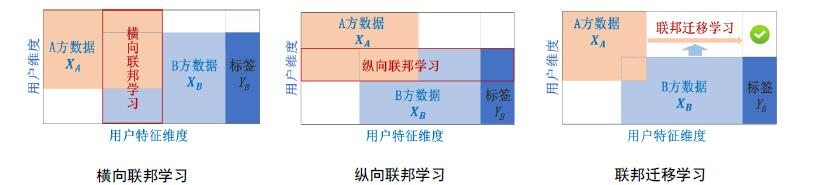
\includegraphics[width=\textwidth]{Categorization_of_FL.jpg}
    \caption{联邦学习的类别}
\end{figure}
\paragraph{横向联邦学习}  横向联邦学习的本质是样本的联合, 适用于参与者间业态相同但客户不同, 即特征重叠多, 用户重叠少时的场景, 比如不同地区的银行间, 他们的业务相似(特征相似), 但用户不同(样本不同).比如有两家不同地区银行, 它们的用户群体分别来自各自所在的地区, 相互的交集很小.但是, 它们的业务很相似, 因此, 记录的用户特征是相同的.此时,  就可以使用横向联邦学习来构建联合模型. 
 
\begin{figure}
    \centering
    \label{Architecture for horizontal FL}
    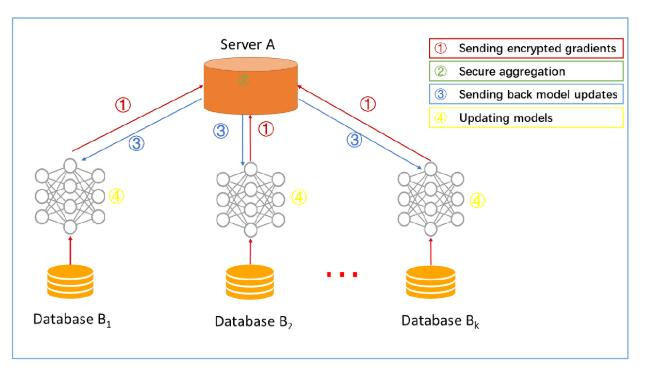
\includegraphics[width=0.9\textwidth]{Architecture_for_horizontal_FL_system.jpg}
    \caption{横向联邦学习的架构}
\end{figure}

\begin{enumerate}
\item 参与者本地计算训练梯度, 使用加密\citep{aono2017privacy}、差异隐私\citep{shokri2015privacy}或秘密共享技术屏蔽梯度\citep{bonawitz2017practical}, 并将屏蔽结果发送给服务器;
\item 服务器在没有关于任何参与者的学习信息的情况下执行安全聚合;
\item 服务器向参与者发送聚合的结果;
\item 参与者更新它们各自的模型具有解密的梯度.
\end{enumerate}

\paragraph{纵向联邦学习}
在两个数据集的用户重叠较多而用户特征重叠较少的情况下, 我们把数据集按照用户维度切分, 并取出双方用户相同而用户特征不完全相同的那部分数据进行训练.比如有两个不同机构, 一家是某地的银行, 另一家是同一个地方的电商.它们的用户群体很有可能包含该地的大部分居民, 因此用户的交集较大.但是, 由于银行记录的都是用户的收支行为与信用评级, 而电商则保有用户的浏览与购买历史, 因此它们的用户特征交集较小.纵向联邦学习就是将这些不同特征在加密的状态下加以聚合, 以增强模型能力的联邦学习.目前, 逻辑回归模型, 树型结构模型和神经网络模型等众多机器学习模型已经逐渐被证实能够建立在这个联邦体系上.


\begin{enumerate}
    \item  第三方C加密样本对齐[9-10].是在系统级做这件事, 因此在企业感知层面不会暴露非交叉用户.
    \item 对齐样本进行模型加密训练
    \begin{itemize}
        \item 由第三方C创建加密数据对, 并且向A和B发送公钥;
        \item A和B分别计算和自己相关的特征中间结果, 并加密交互, 用来求得各自梯度和损失;
        \item A和B分别计算各自加密后的梯度并添加掩码发送给C, 同时B计算加密后的损失发送给C;
        \item C解密梯度和损失后回传给A和B, A、B去除掩码并更新模型.
    \end{itemize}
\end{enumerate}
\paragraph{联邦迁移学习}
在两个数据集的用户与用户特征重叠都较少的情况下, 我们不对数据进行切分, 而可以利用 迁移学习\citep{pan2009survey}来克服数据或标签不足的情况.这种方法叫做联邦迁移学习.\\
比如有两个不同机构, 一家是位于中国的银行, 另一家是位于美国的电商.由于受到地域限制, 这两家机构的用户群体交集很小.同时, 由于机构类型的不同, 二者的数据特征也只有小部分重合.在这种情况下, 要想进行有效的联邦学习, 就必须引入迁移学习, 来解决单边数据规模小和标签样本少的问题, 从而提升模型的效果.
\\
典型的跨设备联邦学习应用程序的数量级大小示意如表\ref{tab:sizes}.
 
\begin{table}
    \centering
    \renewcommand{\arraystretch}{1.2}
    \begin{tabular}{rl}    
    \toprule
    总群体大小 &  $10^6$--$10^{10}$ 设备\\
    为一轮训练选择的设备 & 50 -- 5000 \\
    参与训练一个模型的所有设备 & $10^5$--$10^7$  \\
    模型收敛的轮数 & 500 -- 10000 \\
    wall-colck训练的时间 & 1 -- 10 天 \\ 
    \bottomrule 
    \end{tabular}
    \caption{典型的跨设备联合学习应用程序的数量级大小}
    \label{tab:sizes}
\end{table}


数据中心的联邦学习和分布学习典型特性比较如表\ref{tab:characteristics}.
% Please add the following required packages to your document preamble:
% \usepackage[normalem]{ulem}
% \useunder{\uline}{\ul}{}
% Please add the following required packages to your document preamble:
%
 
\newpage

\newcolumntype{B}[1]{>{\arraybackslash}p{#1}}
\newcolumntype{P}[1]{>{\centering\arraybackslash}p{#1}}

% Widths shold be sum of the B{} widths below plus about 0.1in
\newcommand{\twocolright}[1]{\multicolumn{2}{p{4.1in}}{#1}}
\newcommand{\twocolleft}[1]{\multicolumn{2}{p{3.5in}}{#1}}
\newcommand{\twocolleftcenter}[1]{\multicolumn{2}{P{3.5in}}{#1}}


% \newgeometry{left=0.7in, right=0.7in, top=0.5in, bottom=0.8in}

\begin{table}[t]
    \begin{centering}
    \renewcommand{\arraystretch}{1.5}
    \begin{small}
    \begin{tabular}{@{}B{0.8in}B{1.6in}B{1.8in}B{2.2in}@{}}
    \toprule
     % The \hspaces are a nasty trick to get the line breaks where we want them.
     & \textbf{数据中心\mbox{分布式学习}} & \textbf{Cross-silo\mbox{联邦学习 \hspace{1in}}} & \textbf{跨设备\mbox{联邦学习\hspace{1in}}} \\ 
    \midrule
    设定     
& 在大型但“扁平”的数据集上训练模型.client是单个集群或数据中心中的计算节点.    & 在孤岛式数据上训练模型. client是不同的机构(如医学或金融)或地理分隔的数据中心.
& clients是大量的移动或物联网设备. \\
    
    数据\mbox{分布}
      & 数据是集中存储的, 可以在clients之间转移和平衡.任何client都可以读取数据集的任意部分. 
      & \twocolright{\textbf{ 数据在本地产生并保持去中心化。}每个client存储它自己的数据,并且无法读取其他client的数据。数据并不独立或完全相等地分布。 } \\
    
    编排     
      &中心编排
      & \twocolright{\textbf{由中心服务器(服务)组织模型训练,}但绝对不会看到原始数据} \\
    
    广域通信 \mbox{通信} 
      & 无(clients在一个数据中心/集群中完全连接)
      & \twocolright{星形(hub-and-spoke)拓扑连接,hub代表一个协调服务提供者(通常没有数据),spoke代表与clients的连接} \\
    
      数据 \mbox{可用性 }
      & \twocolleftcenter{\rule[0.8mm]{.6in}{0.4pt}\ 所有clients都几乎一直可用\ \rule[0.8mm]{.6in}{0.4pt}}
      &任何时刻都只有部分client可用,通常受日夜或其他因素影响\\
      分布范围
      &通常有1 - 1000个client.
      &通常有2 - 100个client.
      & 大规模并行, 高达$10^{10}$个client.
      \\
      
      主要\mbox{瓶颈}
      & 数据中心网络很快,瓶颈更多在计算
      & 计算和通信都有可能 
      &        通信一般是主要瓶颈,不过还是取决于任务。通常cross-device联邦计算使用wi-fi或者更慢的连接
      \\
      
      寻址能力
      & \twocolleft{每个client都有一个id或名称,系统可以明确地找到它}
      &client不能被直接素引〔不能使用client的id)
      \\
      
      client\mbox{有状态性}
      & \twocolleft{有状态 —— 每个client都可能参与到每一轮通信中,在各轮中都带有状态      }
      &没有状态 —— 每个client都很可能在一个任务中只参与一次,所以通常假定会有在之前的通信中从没见过的全新样本
      \\
      
      client\mbox{可靠性}
      & \twocolleftcenter{\rule[0.8mm]{1.0in}{0.4pt} \ 相对较少的失败.
      \ \rule[0.8mm]{1.0in}{0.4pt} }
      &非常不可靠 —— 5\%或更多的参与一轮让算的client可能会失败或推出(例如设备由于违反电池、网络、或者而空闲率要求而不合格).
      \\
      
      数据分区轴
      &数据可以在clients之间被任意partition和repartition
& partition固定,可能按样本(横向)或按特征(纵向)partition
      & partition是固定的,并且是按样本横向\\ 
    
    \bottomrule
    \end{tabular}
    \end{small}
    \caption{典型特征联邦学习设置与数据中心的分布式学习(例如\citep{dean2012large}). 跨设备和cross-silo跨孤井联邦学习是联邦学习领域的两个例子, 但并不是详尽的.}
    \label{tab:characteristics}
    \end{centering}
    \end{table}
  
    \subsubsection{联邦学习中模型的生命周期}
    \begin{figure}[ht]
        \setlength{\abovecaptionskip}{0.1cm}
        \centering    
        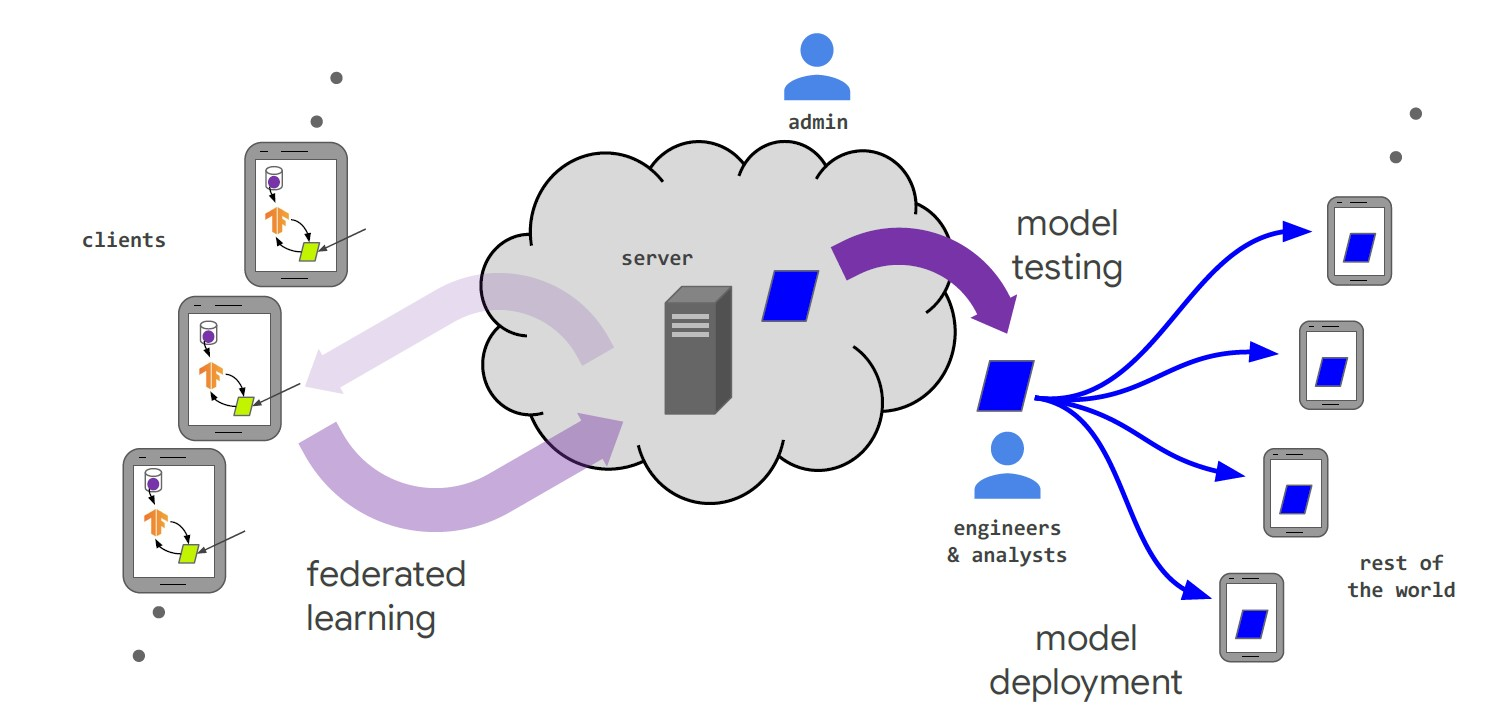
\includegraphics[width=0.6\textwidth]{life_circle.jpg}
        \caption{联邦学习中模型的生命周期}
    \end{figure}
在联邦学习过程中, 模型的生命周期通常由为特定应用程序开发模型的模型工程师驱动.例如, 自然语言处理领域的专家可以开发用于虚拟键盘的下一个单词预测模型.图1显示了主要组件和参与者.在高层, 一个典型的工作流程是:
\begin{enumerate}
\item	\textbf{问题识别:}\ 模型工程师识别出一个需要用FL解决的问题.
\item	\textbf{客户端插装:} \ 如果需要, 客户端(例如在移动电话上运行的应用程序)被插装到本地存储(有时间和数量限制)必要的训练数据.在许多情况下, 应用程序已经存储了这些数据(例如, 一个文本消息应用程序必须存储文本消息, 一个照片管理应用程序已经存储了照片).然而, 在某些情况下, 可能需要维护额外的数据或元数据, 例如用户交互数据来为监督学习任务提供标签.
\item	\textbf{仿真原型(可选):} \ 模型工程师可以在一个使用代理数据集的FL仿真中原型模型架构和测试学习超参数.
\item	\textbf{联邦模型训练:} \ 启动多个联邦训练任务来训练模型的不同变体, 或使用不同的优化超参数.
\item	\textbf{(联邦)模型评估:} \ 在任务得到充分训练(通常是几天, 见下文)之后, 分析模型并选择合适的候选者.分析可能包括在数据中心的标准数据集上计算的度量, 或者联合评估, 在联合评估中, 模型被推送到指定的客户端, 以对本地客户端数据进行评估.
\item	\textbf{部署:} \ 最后, 一旦选择了一个好的模型, 它通过一个标准模型发布过程, 包括人工质量保证, 在线A/B测试(通常通过使用新模型在一些设备和其他设备来比较他们的上一代模型体内性能), 并分阶段推出(以便于发现表现差的行为并且在影响太多的用户之前回退).模型的特定启动过程由应用程序的所有者设置, 通常与模型的训练方式无关.
\end{enumerate}
 
\subsubsection{典型的联邦训练过程}
我们现在考虑一个FL训练模板, 它包含McMahan等人\citep{mcmahan2016communication}和许多其他人的联邦平均算法;同样, 可能会有变化, 但这提供了一个共同的起点.
服务器(服务提供商)通过重复以下步骤来编排训练过程, 直到训练停止(由监控训练过程的模型工程师决定):


\begin{enumerate}
\item 客户端选择:服务器从一组满足资格要求的客户端取样.例如, 为了避免影响设备的用户, 移动电话可能只有在接入无线网络并处于空闲状态时才会登录到服务器.
\item 广播:选定的客户端从服务器下载当前模型的权值和一个训练程序(例如一个TensorFlow图表[6]).
\item 客户端计算:每个选择的设备通过执行训练程序在本地计算对模型的更新, 例如可以在本地数据上运行SGD(如联合平均).
\item 聚合:服务器收集设备更新的聚合.为了提高效率, 一旦有足够数量的设备报告了结果, 掉队者可能会被丢弃.此阶段也是许多其他技术的集成点, 稍后将讨论这些技术, 可能包括:用于增加隐私的安全聚合、用于提高通信效率的聚合的有损压缩, 以及用于差异隐私的噪声添加和更新裁剪.
\item 模型更新:服务器根据从参与当前轮的客户机计算的聚合更新, 在本地更新共享模型.
\end{enumerate}
表2给出了移动设备上典型的联邦学习应用程序所涉及的数量的典型数量级大小.

%%
%这一部分你可以根据你对论文的理解进一步提炼.关于该问题目前研究的进展是什么?目前已有哪些工作?这些工作之间的发展脉络是什么?

\subsection{联邦学习研究} 

联邦学习和完全去中心化学习的主要区别比较如表\ref{tab:decentralized}.
注意使用联邦学习, 去中心化学习可以进一步划分为不同的用例.
\begin{table}
    \begin{centering}
    \renewcommand{\arraystretch}{1.5}
    \begin{tabularx}{\textwidth}{lXX}
    \toprule
           & \textbf{联邦学习} & \textbf{完全去中心化(端对端学习)} \\
    \midrule  
编排
&中心业务流程服务器或服务组织训练, 但从不查看原始数据.
&没有集中的业务流程.
\\
广域通信
& hub-and-spoke拓扑, 其中hub表示协调服务提供者(通常没有数据), 而spoke节点连接到客户端.
&点对点拓扑, 可能是动态连接图.
\\ 
    \bottomrule
    \end{tabularx}
    \caption{联邦学习和完全去中心化学习的主要区别}
    \label{tab:decentralized}
    \end{centering}
\end{table}
 
\subsubsection{Cross-soli联邦学习} 
与跨设备联合学习的特征相反,  跨孤井Cross-Silo联邦学习在总体设计的某些方面非常灵活.许多组织如果只是想共享训练模型, 而不想分享数据时, cross-silo设置是非常好的选择.Cross-Silo 联邦学习的设置主要有以下几个要点:数据分割、激励机制、.差异隐私、张量因子分解.


分割学习(Split Learning):分割学习的关键思想是在客户端和服务器之间执行基于每层的分割模型, 并应用于训练和推理.分裂学习最简单配置是每个客户端计算通过深层网络前向传递, 然后切割层的输出, 即粉碎数据被发送到另一个服务器或客户端, 然后由此服务器或客户端完成剩余的计算.这意味着让不共享的数据发生前向传播;最后可以以类似的方式将梯度从其最后一层反向传播到切割层.注意此过程会一直持续到收敛.
\begin{figure}[ht]
    \centering    
    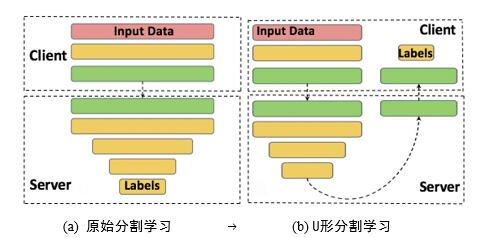
\includegraphics[width=0.6\textwidth]{split_learning.jpg}
    \caption{分割学习}
\end{figure}


分割学习(Split learning)的关键思想, 与之前着重于数据分区和通信模式的设置相比, 它是在客户端和服务器之间按层划分执行模型, 这对于训练和推理都是一样的.
如图所示:(a)在普通拆分学习的设置, 原始数据不会传输;(b)在U-形拆分学习的设置, 在客户端和服务器实体之间原始数据和标签不会传输.



\subsubsection{算法挑战}



联邦学习的核心是谷歌在其论文\cite{mcmahan2016communication}中引入的联邦平均算法\cite{alg:fedavg}. 
 

   \begin{algorithm}[t]
    \begin{algorithmic}
    \State \textbf{Server executes:}
       \State initialize $w_0$
       \FOR{each round $t = 1,  2,  \dots$} 
       \hspace{1em} \State $m \leftarrow \max( C\cdot K,  1)$
          \State $S_t \leftarrow$ (random set of $m$ clients)
           \FOR{each client $k \in S_t$ \textbf{in parallel}}
            \State $w_{t+1}^k \leftarrow \text{ClientUpdate}(k,  w_t)$ 
           \State $w_{t+1} \leftarrow \sum_{k=1}^K \frac{n_k}{n} w_{t+1}^k$ \\

     \State {\textbf{ClientUpdate}($k,  w$):}\ \ \  // \emph{Run on client $k$}
      \State $\mathcal{B} \leftarrow$ (split $\mathcal{P}_k$ into batches of size $\lbs$)
       \FOR{each local epoch $i$ from $1$ to $ \lepochs$}
      \FOR{batch $b \in \mathcal{B}$}
         \State $w \leftarrow w - \eta \nabla \ell(w; b)$
       \State return $w$ to server
    \end{algorithmic}
    \caption{FederatedAveraging. The $K$
      clients are indexed by $k$; $\lbs$ is the local minibatch size, 
      $\lepochs$ is the number of local epochs,  and $\eta$ is the learning
      rate.} 
    \label{alg:fedavg}
    \end{algorithm}
     
    \begin{description}
        \item[Step1:] 选择成员的一个随机子集(称为客户机)以同步方式从服务器接收全局模型. 
        \item[Step2:] 每个选择的客户端使用其本地数据计算一个更新的模型. 
        \item[Step3:] 模型更新从选择的客户端发送到服务器.  
        \item[Step4:] 服务器聚合这些模型(通常通过平均)来构建一个改进的全局模型.  
    \end{description}

子集选择步骤是谷歌最初应用联邦学习的环境所必需的:\textbf{基于在其Android生态系统中通过数百万部手机收集的数据}. 这种学习序列的一种变体出现在之后的论文中, 包括发送梯度更新到服务器, 而不是实际的模型权重本身. 通常, 在各方之间不传输任何原始数据, 只传输与模型相关的更新. \textbf{边缘计算}在这里体现出作用. 
 
在机器学习分散方案的现实可用性问题上, 许多重要的算法问题仍然没有解决.有些问题类似于使用中央服务器进行联合学习的特殊情况, 而其他挑战则是完全分散或不信任的额外副作用.如
\begin{itemize}
    
\item 网络拓扑结构和异步性对去中心化SGD的影响
\item 本地更新对与中心化SGD
\item 个性化和信任机制
\item 梯度压缩和量化方法
\end{itemize}

\paragraph{}
 
    \subsubsection{实际挑战}

今天的区块链平台数据在默认情况下, 可能会阻止用户参与联邦分割学习.

解决方案:
为了防止参与节点利用单独提交的模型更新, 可以使用现有的安全聚合协议.

为了防止任何客户机试图重建另一个客户的私人数据利用全球模型, 客户级差分隐私[290]已被提议用于FL.客户级差分隐私是通过在聚合的全局模型上添加随机高斯噪声来实现的, 该噪声足以隐藏任何单个客户端的更新.

\paragraph{推理攻击} 联邦学习的动机是保护客户拥有的数据的隐私. 即使没有公开实际数据, 也可以利用重复的模型权重更新来揭示对数据而言不是全局的而是特定于各个贡献者的属性. 可以在服务器端以及(其他)客户端端执行此推断. 通常引用的对策是使用差异隐私来减轻这种风险. 

\paragraph{模型中毒Model Poisoning}. 一些研究人员研究了使客户误导后门功能或进行Sybil攻击以毒害全局模型的可能性. 
 \textbf{Sybil} 攻击:允许客户端加入和离开的系统容易受到sybil攻击, 在这种攻击中, 对手通过使用多个串通的别名加入一个系统来获得影响力. 
\begin{figure}[t]
    \centering    
    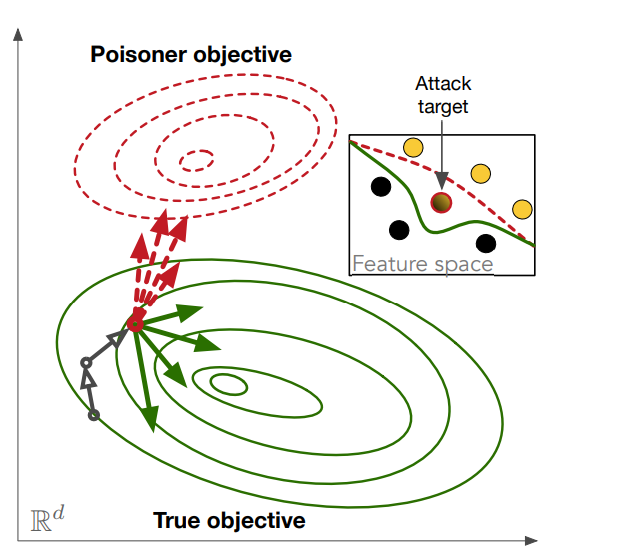
\includegraphics[width=0.6\textwidth]{poisoninginSGD.png}
    \caption{Targeted poisoning attack in SGD. 红色点的矢量是Sybil的贡献, 推动模型走向一个中毒的目标. 坚实的绿色载体是由诚实的客户贡献的, 推动到达真正的目标.     }
\end{figure}
为了有效应对此类攻击, 必须考虑Sybil检测的额外开销. 